\documentclass{article} % For LaTeX2e
\usepackage{nips13submit_e,times}
\usepackage{hyperref}
\usepackage{url}
\usepackage{graphicx}
\usepackage{hyperref}
\graphicspath{ {images/} }
%\documentstyle[nips13submit_09,times,art10]{article} % For LaTeX 2.09


\title{Clustering Wikipedia Articles}


\author{
Lane Aasen\\
Department of Computer Science\\
University of Washington\\
Seattle, WA 98105\\
\texttt{aaasen@cs.washington.edu}\\
}

% The \author macro works with any number of authors. There are two commands
% used to separate the names and addresses of multiple authors: \And and \AND.
%
% Using \And between authors leaves it to \LaTeX{} to determine where to break
% the lines. Using \AND forces a linebreak at that point. So, if \LaTeX{}
% puts 3 of 4 authors names on the first line, and the last on the second
% line, try using \AND instead of \And before the third author name.

\newcommand{\fix}{\marginpar{FIX}}
\newcommand{\new}{\marginpar{NEW}}

\nipsfinalcopy % Uncomment for camera-ready version

\begin{document}


\maketitle

\begin{abstract}
Clustering Wikipedia articles using K-Means. Exploration into K-Means including choice of K, K-Means++, the effect of random seeds, and tf-idf thresholds.
\end{abstract}


\section{Dataset}

The provided dataset contains 15,903 Wikipedia articles in term frequency inverse document frequency (tf-idf) format. Most of the articles are in English, but some are not. Sorting the documents by language would be an interesting project in itself! There are 10,574 unique words in this dataset. Each document is represented as a sparse vector with one dimension for each word. Stop words have been removed from the dataset, but uncommon words remain.

\section{K-Means Clustering}

My first goal was to implement a basic K-Means clustering algorithm from scratch. The code is available at \url{https://github.com/aaasen/wiki-cluster}.

\subsection{Choosing K}

\subsubsection{Minimizing Distortion}

Given $K$ clusters $C_{1},C_{2},...,C_{K}$ where each cluster is a set of document vectors and $\mu_{i}$ is the centroid of $C_{i}$, the total distortion is defined as follows:

$$\sum_{i=1}^{K}\sum_{d \in C_{i}} ||d - \mu_{i}||^{2}$$

To minimize the distortion, we could set $K$ equal to the number of documents, but then the clusters would be meaningless. We want to choose a $K$ with low distortion that also results in interpretable clusters. Figure 1 shows a plot of $K$ versus total distortion. When $1 \leq K \leq 16$, adding additional clusters has a large impact on the distortion, but once $K > 16$, adding additional clusters has little impact on the distortion. From this alone, it makes sense to set $K=16$ since it provides a good balance of distortion and interpretability.

\clearpage

\begin{figure}[h]
\begin{center}
\framebox{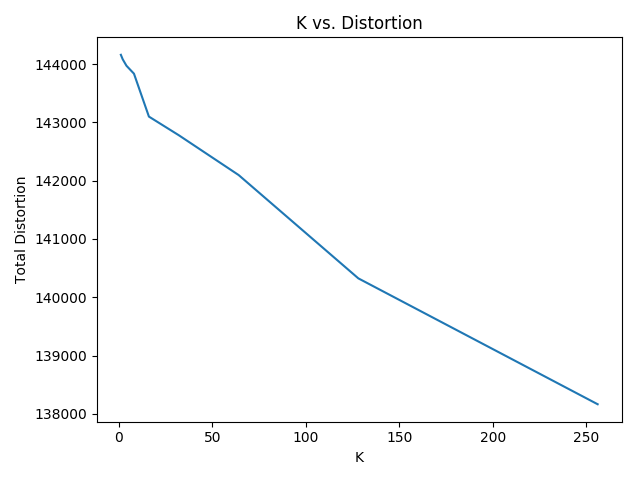
\includegraphics[scale=0.4]{k_vs_distortion}}
\end{center}
\caption{$K$ versus total distortion for $K \in \{1,2,4,...,256\}$}
\end{figure}

\subsection{K and Cluster Size}

As $K$ increases, the clusters become more sparse. Once $K=256$, over half of the clusters have only one document, and are essentially useless. When $K=16$, the median cluster size is 8.5, and the cluster sizes are as follows:

$$[10061, 3013, 1128, 909, 707, 30, 23, 13, 4, 4, 3, 2, 2, 2, 1, 1]$$

Over half of the clusters are very small, and one of the clusters is too large to be interpretable. This indicates that the data has significant outliers and may lack a structure conducive to clustering.

\begin{figure}[h]
\begin{center}
\framebox{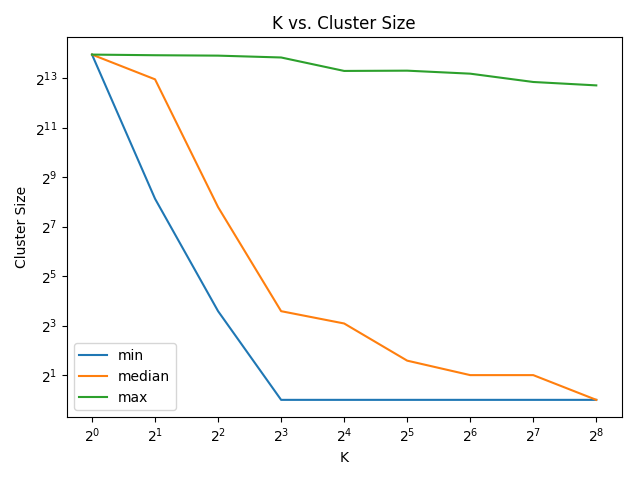
\includegraphics[scale=0.4]{k_vs_cluster_size}}
\end{center}
\caption{$K$ versus minimum, median, and maximum cluster size for $K \in \{1,2,4,...,256\}$ with a $log_{2}$ scale on both axes.}
\end{figure}

\subsection{Exploring Clusters}

Table 1 shows the clusters with at least 10 documents for K-Means clustering with $K=16$. The words in each cluster are the dimensions of the centroid with the largest magnitude. The documents shown are those that are closest to the centroid of the cluster. 

Overall, the generated clusters make sense, but there are some points of confusion:

\begin{itemize}
\item The words that make up cluster 0 have little relation to each other. This cluster contains the majority of the documents.
\item Cluster 1 contains churches as well as colleges.
\item Cluster 3 contains documents related to TV shows and sports because both contain the word "season." Another explanation for this is that sports players appear on Dancing with the Stars.
\end{itemize}



\begin{table}[!htb]
\caption{K-Means clusters with $K=16$ and at least 10 documents.}
\label{cluster-table}
\begin{center}
    \begin{tabular}{ | c | c | c | c |}
    \hline
    \textbf{Cluster} & \textbf{Size} & \textbf{Words} & \textbf{Documents} \\ \hline
    
0 & 10061 & \parbox[t]{2cm}{females \\ station \\ family \\ located \\ north} & \parbox[t]{8cm}{mcgillpainquestionnaire \\ historyofthefamily \\ thetussaudsgroup \\ nadiraactress \\ mansfieldsummithighschool} \\ \hline 
1 & 3013 & \parbox[t]{2cm}{church \\ college \\ students \\ published \\ institute} & \parbox[t]{8cm}{edmondscommunitycollege \\ helderbergcollege \\ oberlincongregationalchurch \\ lundbyoldchurch \\ dioceseoflimerickandkillaloe} \\ \hline 
2 & 1128 & \parbox[t]{2cm}{party \\ served \\ general \\ member \\ senate} & \parbox[t]{8cm}{partyidentification \\ labourfarmerparty \\ democraticalliancesouthafrica \\ liberaldemocratsitaly \\ christiancreditparty} \\ \hline 
3 & 909 & \parbox[t]{2cm}{season \\ club \\ playing \\ seasons \\ player} & \parbox[t]{8cm}{dancingwiththestars \\ davidmccracken \\ gilbertcurgenven \\ bjsamsamericanfootball \\ livingstonewalker} \\ \hline 
4 & 707 & \parbox[t]{2cm}{album \\ released \\ songs \\ records \\ rock} & \parbox[t]{8cm}{thegreatestdaytakethatalbum \\ conflictingemotions \\ primalscream \\ leftbacklp \\ elisamartin} \\ \hline 
5 & 30 & \parbox[t]{2cm}{nba \\ basketball \\ points \\ season \\ seasons} & \parbox[t]{8cm}{kcjones \\ hakeemolajuwon \\ albertkingbasketball \\ ballstatecardinalsmensbasketball \\ 201011southfloridabullsmensbasketballteam} \\ \hline 
6 & 23 & \parbox[t]{2cm}{riots \\ police \\ murder \\ captured \\ robbery} & \parbox[t]{8cm}{sowetouprising \\ 1992losangelesriots \\ nikolaybogolepov \\ josephlamothe \\ jenmi} \\ \hline 
7 & 13 & \parbox[t]{2cm}{congo \\ subtropical \\ republic \\ zambia \\ zimbabwe} & \parbox[t]{8cm}{republicofcabinda \\ brownrumpedbunting \\ copperbeltprovince \\ leptopelisviridis \\ yellowthroatedpetronia} \\ \hline 
 
\end{tabular}
\end{center}
\end{table}

\subsection{K-Means++}

K-Means++ is a method for selecting the initial cluster centers for K-Means. In the normal version of K-Means, initial cluster centroids are selected by sampling random documents from the dataset. This can produce suboptimal clusters, increase time to convergence, and increase variability in clustering performance. 

K-Means++ solves this by selecting initial centroids one at a time in order to minimize distortion. Each document is given a weight proportional to the distance to the nearest centroid and the next centroid is selected at random using these weights until $K$ centroids have been chosen. This results in better centroids than random sampling and lessens the time until convergence. However, it can be quite expensive when $K$ is large since the distance from each document to each cluster centroid must be computed at every iteration.

I implemented K-Means++ and expected it to increase clustering performance considerably. However, I found that it actually had a slightly negative impact on distortion and noticeably increased cluster sparsity. 

I think that this is because outliers were chosen as initial centroids and the clusters never expanded to include other points.

\begin{figure}[h]
\begin{center}
\framebox{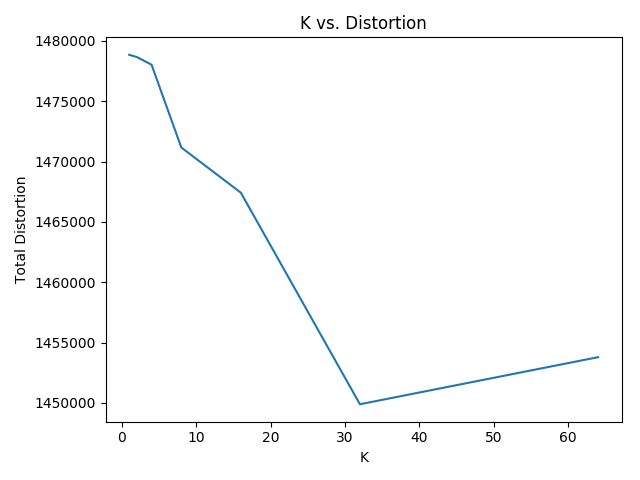
\includegraphics[scale=0.4]{k_vs_distortion_++}}
\end{center}
\caption{$K$ versus total distortion for $K \in \{1,2,4,...,64\}$ using K-Means++.}
\end{figure}


\begin{figure}[h]
\begin{center}
\framebox{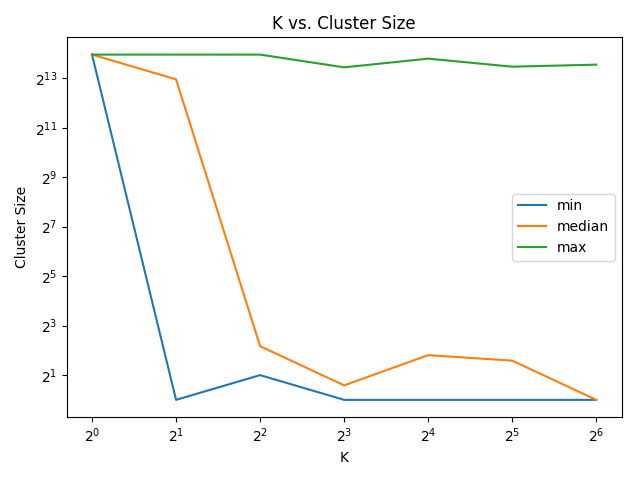
\includegraphics[scale=0.4]{k_vs_cluster_size_++}}
\end{center}
\caption{$K$ versus minimum, median, and maximum cluster size for $K \in \{1,2,4,...,64\}$ with a $log_{2}$ scale on both axes. Using K-Means++.}
\end{figure}

\subsection{Fighting Cluster Sparsity}

After implementing K-Means++ with no success, it became apparent that there was a problem with the underlying data, and not with the clustering algorithm. 

I began to investigate the provided dataset, which was in tf-idf format with no documentation. I found that stop words had been removed from the dataset, but rare words had been left in. Half of the words in the dictionary were used in 16 or fewer datasets (less than 0.1\%). Tables 2, 3, and 4 show the least common, somewhat common, and most common words in the dataset, respectively.

\begin{table}[t]
\caption{10 least common words with the number and percentage of documents that they appear in.}
\label{least-common-words-table}
\begin{center}
    \begin{tabular}{ | c | c | c |}
    \hline
    \textbf{Word} & \textbf{Documents} & \textbf{Percentage of Documents} \\ \hline

frazioni & 0 & 0.0\% \\ \hline 
threeletter & 1 & 0.0062881\% \\ \hline 
budjovice & 1 & 0.0062881\% \\ \hline 
gmina & 1 & 0.0062881\% \\ \hline 
ortsgemeinden & 1 & 0.0062881\% \\ \hline 
headwater & 2 & 0.012576\% \\ \hline 
baronetage & 3 & 0.018864\% \\ \hline 
breaststroke & 3 & 0.018864\% \\ \hline 
voronezh & 3 & 0.018864\% \\ \hline 
rosettes & 3 & 0.018864\% \\ \hline 

\end{tabular}
\end{center}
\end{table}


\begin{table}[t]
\caption{10 words near the median with the number and percentage of documents that they appear in.}
\label{median-common-words-table}
\begin{center}
    \begin{tabular}{ | c | c | c |}
    \hline
    \textbf{Word} & \textbf{Documents} & \textbf{Percentage of Documents} \\ \hline

multimillion & 16 & 0.10061\% \\ \hline 
pisa & 16 & 0.10061\% \\ \hline 
pranks & 16 & 0.10061\% \\ \hline 
pesticides & 16 & 0.10061\% \\ \hline 
hesitation & 16 & 0.10061\% \\ \hline 
convection & 16 & 0.10061\% \\ \hline 
ortiz & 16 & 0.10061\% \\ \hline 
stagnation & 16 & 0.10061\% \\ \hline 
gonzlez & 16 & 0.10061\% \\ \hline 
cummins & 16 & 0.10061\% \\ \hline 

\end{tabular}
\end{center}
\end{table}

\begin{table}[!htb]
\caption{10 most common words with the number and percentage of documents that they appear in.}
\label{most-common-words-table}
\begin{center}
    \begin{tabular}{ | c | c | c |}
    \hline
    \textbf{Word} & \textbf{Documents} & \textbf{Percentage of Documents} \\ \hline

well & 4009 & 25.209\% \\ \hline 
second & 3538 & 22.247\% \\ \hline 
high & 2836 & 17.833\% \\ \hline 
family & 2579 & 16.217\% \\ \hline 
group & 2412 & 15.167\% \\ \hline 
north & 2364 & 14.865\% \\ \hline 
major & 2298 & 14.45\% \\ \hline 
large & 2227 & 14.004\% \\ \hline 
general & 2187 & 13.752\% \\ \hline 
long & 2164 & 13.607\% \\ \hline 

\end{tabular}
\end{center}
\end{table}



\subsubsection{Selecting a Threshold}

Since the provided dataset does not contain stop words, I decided not to filter out common words. The most common words in the dataset appear to contain useful information for clustering. 

Selecting a lower threshold involves finding the right balance between information loss and cluster sparsity. Words that are only used in one document should be ignored since they provide no useful clustering information. The problem gets murkier with words that are used in just a few datasets. Table 3 lists ten words that are somewhat common, in that their counts are exactly at the median word count. Some of these words seem useful for clustering, such as "multimillion", "pesticides", and "convection". Others are names which do not necessarily indicate document similarity. 

One of the large problems here is that we are working with only 15,000 of the 5 million English Wikipedia articles. If we were working with more data, we could produce more fine-grained clusters with rarer words. However, since we only have a tiny subset of Wikipedia, we just don't have enough examples to produce these narrow clusters.

There is no correct way to choose a tf-idf threshold. I ended up choosing to get rid of the least common half of words, but many other choices would be just as valid.




\subsection{Effect of Seed on Distortion}

After observing some unexpected variability in my results, I decided to investigate the effect of random seeds on distortion.

I found that the choice of seed can have a large impact on cluster quality and distortion. Because of this, it is very important to run K-Means with at least a few different seeds and select the best one. While this can be too computationally expensive to do when running experiments, it is important to do when generating the final clusters.

\begin{figure}[h]
\begin{center}
\framebox{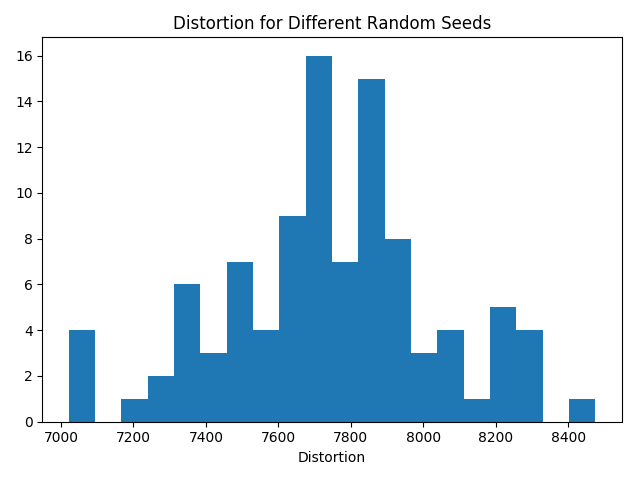
\includegraphics[scale=0.4]{different_init}}
\end{center}
\caption{Distortion using K-Means++ on 100 training documents with different random seeds.}
\end{figure}

\section{Conclusion}

Table 5 shows the final clusters. While 64 clusters were generated, only the largest 10 are shown. Only words that occurred in at least 16 documents, which is about half of all words, were considered. K-Means++ was used to generate the initial cluster centroids. Names have been added to each cluster.
 
\subsection{Issues with K-Means}

\subsubsection{Variability in Cluster Size}

The most glaring issue with these results is that the sizes of the clusters vary greatly. One cluster contains about half of the documents while the other 63 contain the other half. There are many useless one document clusters.

It is difficult to know if this is an intrinsic part of the data, or an issue with the K-Means algorithm. I suspect that it is a combination of both, and that K-Means is not the best model for the data.

While exploring the data, I did try to visualize it using Multidimensional Scaling (MDS), but I found that too much information was lost in the dimensionality reduction for it to be of any use. Textual data is high dimensional and sparse by its nature, which makes it somewhat unintuitive to work with in this context. It would be interesting to further explore dimensionality reduction techniques as well as alternate clustering algorithms and see if they could help address the problem of cluster sparsity.

\subsubsection{Different Meanings of the Same Word}

Some clusters contain documents that are related by a single word, where each document refers to a different meaning of the word. For example, cluster 9 contains documents about mars. Its main words are "mars", "crater", "astronomical", "expedition", and "planets". However, there are two documents in this cluster that have nothing to do with mars. "hostagefilm" (\textit{Hostage} (film)) is an American action movie whose main character is named Marshall "Mars" Krupcheck. "marsrapper" (\textit{Mars} (rapper)) is a Bay Area rapper who goes by "Mars".


\subsection{Further Research}

I had intended to explore Latent Dirichlet Allocation but ended up focusing on K-Means instead. As a starting point, I used SciKit's LDA implementation, which seemed to work quite well. The words in each topic are related just as they should be. This would have been be a great topic to research more, if I had the time.

\begin{table}[!htb]
\caption{16 topics generated using Latent Dirichlet Allocation.}
\label{most-common-words-table}
\begin{center}
    \begin{tabular}{ | c | }
    \hline
    \textbf{Topics} \\ \hline

magazine, published, journal, format, awards \\ \hline 
painting, gallery, paintings, painted, station \\ \hline 
greek, empire, ancient, jews, dynasty \\ \hline 
served, appointed, general, senate, member \\ \hline 
systems, system, design, device, czech \\ \hline 
party, security, elections, rights, police \\ \hline 
station, air, route, railway, traffic \\ \hline 
season, females, club, miles, tournament \\ \hline 
church, building, house, located, castle \\ \hline 
group, swedish, users, stockholm, program \\ \hline 
engine, cars, comics, ford, novels \\ \hline 
students, college, institute, campus, program \\ \hline 
player, characters, red, color, blue \\ \hline 
album, released, songs, musical, records \\ \hline 
human, family, published, man, god \\ \hline 
common, temperature, chemical, protein, oil \\ \hline 

\end{tabular}
\end{center}
\end{table}





\begin{table}[!b]
\caption{10 largest K-Means clusters with $K=64$. Using words that appear in at least 16 (0.1\%) documents with K-Means++ for initializing cluster centroids.}
\label{cluster-new-table}
\begin{center}
    \begin{tabular}{ | c | c | c | c | c | }
    \hline
    \textbf{Cluster} & \textbf{Size} & \textbf{Words} & \textbf{Documents} & \textbf{Label} \\ \hline
 
0 & 8486 & \parbox[t]{2cm}{females \\ station \\ family \\ north \\ located} & \parbox[t]{5cm}{kotavamsa \\ tornadoesof1993 \\ whitby \\ colinmeads \\ mladeniiiubiofbribir} &  \\ \hline 
1 & 2226 & \parbox[t]{2cm}{students \\ system \\ high \\ program \\ technology} & \parbox[t]{5cm}{edmondscommunitycollege \\ helderbergcollege \\ stargateschool \\ miltonhighschoolmiltongeorgia \\ govthazimuhammadmohsincollege} & Colleges \\ \hline 
2 & 2085 & \parbox[t]{2cm}{church \\ published \\ daughter \\ royal \\ paris} & \parbox[t]{5cm}{molire \\ oberlincongregationalchurch \\ lundbyoldchurch \\ stmaryschurchgrodno \\ dioceseoflimerickandkillaloe} & Churches \\ \hline 
3 & 1001 & \parbox[t]{2cm}{party \\ served \\ member \\ general \\ senate} & \parbox[t]{5cm}{partyidentification \\ labourfarmerparty \\ serbianliberalparty \\ bronwenmaher \\ democraticalliancesouthafrica} & Political Parties \\ \hline 
4 & 932 & \parbox[t]{2cm}{season \\ club \\ playing \\ seasons \\ player} & \parbox[t]{5cm}{bjsamsamericanfootball \\ dancingwiththestars \\ davidmccracken \\ johnflanaganfootballer \\ gilbertcurgenven} & Sports \\\hline 
5 & 640 & \parbox[t]{2cm}{album \\ released \\ songs \\ records \\ rock} & \parbox[t]{5cm}{primalscream \\ thegreatestdaytakethatalbum \\ conflictingemotions \\ bornthisway \\ sweetkisses} & Rock Music \\ \hline 
6 & 280 & \parbox[t]{2cm}{japanese \\ japan \\ chinese \\ pearl \\ characters} & \parbox[t]{5cm}{frederickringer \\ astorhousehotelshanghai19221959 \\ japanesebadger \\ imperialjapanesearmyairforce \\ listofflclepisodes} & Imperial Japan \\ \hline 
7 & 44 & \parbox[t]{2cm}{pop \\ songs \\ album \\ chart \\ rock} & \parbox[t]{5cm}{popmusic \\ teenpop \\ britishpopmusic \\ talkinginyoursleepcrystalgaylesong \\ blahblahblahalbum} & Pop Music \\ \hline 
8 & 27 & \parbox[t]{2cm}{investigation \\ money \\ system \\ june \\ doctor} & \parbox[t]{5cm}{digitalmonetarytrust \\ andyhayman \\ martensvillesatanicsexscandal \\ johnlittlechild \\ unitedstatesvlibby} & Crime \\ \hline 
9 & 22 & \parbox[t]{2cm}{mars \\ crater \\ astronomical \\ expedition \\ planets} & \parbox[t]{5cm}{hostagefilm \\ marsrapper \\ entomopter \\ mars2 \\ carbonatesonmars} & Mars \\ \hline 
 
\end{tabular}
\end{center}
\end{table}

\clearpage

\subsubsection*{References}

\small{
[1] MacQueen, J. B. (1967). Some Methods for classification and Analysis of Multivariate Observations. {\it Proceedings of 5th Berkeley Symposium on Mathematical Statistics and Probability }. 1. University of California Press. pp. 281–297. MR 0214227. Zbl 0214.46201. Retrieved 2009-04-07.

[2] Arthur, D.; Vassilvitskii, S. (2007). "k-means++: the advantages of careful seeding" (PDF). {\it Proceedings of the eighteenth annual ACM-SIAM symposium on Discrete algorithms.} Society for Industrial and Applied Mathematics Philadelphia, PA, USA. pp. 1027–1035.
}

\end{document}